\documentclass[12pt]{article}
\usepackage[utf8]{inputenc}
\usepackage{ucs}
\usepackage{amsmath} 
\usepackage{mathtext}
\usepackage{amsfonts}
\usepackage{upgreek}
\usepackage[english,russian]{babel}
\usepackage{graphicx}
\usepackage{float}
\usepackage{textcomp}
\usepackage{hyperref}
\usepackage{geometry}
  \geometry{left=2cm}
  \geometry{right=1.5cm}
  \geometry{top=1cm}
  \geometry{bottom=2cm}
\usepackage{tikz}
\usepackage{ccaption}
\usepackage{float}
\usepackage{verbatim}
\restylefloat{table}


\begin{document}
\pagenumbering{gobble}

\section*{Графы}
\subsection*{Часть А}

\begin{enumerate}
\item \textbf{Матрица смежности} Решить задачу graph\_1 на ejudge.
\item \textbf{Список ребер} Решить задачу graph\_2 на ejudge.
\item \textbf{Создание графа} На этом семинаре мы воспользуемся уже готовой реализацией графа, которая расположена в папке ./code/graph (или по адресу \\ \href{github.com/v-biryukov/cs_mipt_faki/tree/master/term2/seminar1_graph/code/graph}{github.com/v-biryukov/cs\_mipt\_faki/tree/master/term2/seminar1\_graph/code/graph})
В файлах graph.h и graph.c реализована структура данных граф, а в файлах search.h и search.c реализованы поиск в глубину(dfs) и поиск в ширину(bfs).
В файле main\_graph.c приведён пример использования этой реализации графа. Например, следующий участок кода создаёт и инициализирует граф.
\begin{verbatim}
    g = graph_create(10);
    for(i = 0; i < 10; i++) {
        graph_add_edge(g, i, (i + 1) % 10);
        graph_add_edge(g, (i + 1) % 10, i);
    }
    graph_add_edge(g, 3, 7);
    graph_add_edge(g, 6, 2);
\end{verbatim}.
\begin{itemize}
\item Нарисуйте граф инициализованный в этом файле.
\item Скомпилируйте и запустите программу.
\item Инициализируйте графы, изображённые на рисунках
\begin{figure}[H]
    \centering
    \begin{minipage}{0.4\textwidth}
        \centering
        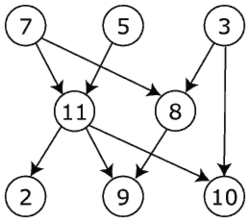
\includegraphics[width=0.8\textwidth]{simple_graph2} % first figure itself
    \end{minipage}\hfill
    \begin{minipage}{0.4\textwidth}
        \centering
        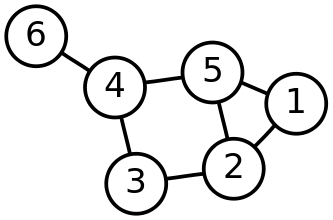
\includegraphics[width=0.8\textwidth]{simple_graph} % second figure itself
    \end{minipage}
\end{figure}
\end{itemize}

\item \textbf{Очередь с приоритетом} (англ. priority queue) -- абстрактный тип данных в программировании, поддерживающий две обязательные операции добавить элемент и извлечь минимум. Очередь с приоритетом похожа на обычные стек и очередь, только элементы из неё извлекаются в том порядке в котором они пришли, а в соответствии с некоторым приоритетом, например, величиной ключа элемента. Асимптотические сложности вставки и извлечения минимального элемента зависят от реализации очереди с приоритетом. Для простой реализации с помощью кучи(heap) эти сложности равны $O(log(n))$. \\
Очередь с приоритетом реализована в файлах pq.c и pq.h.
\begin{itemize}
\item В файле pq.h описаны прототипы функций, созданных для работы с очередью с приоритетом. Вам нужно, пользуясь только этой информацией, понять как работает данная реализация очереди с приоритетом.
\item Использую очередь с приоритетом, можно просто написать ещё один алгоритм сортировки. Придумаёте как это сделать и напишите данную сортировку.
\item Оцените ассимптотическую сложность данного алгоритма сортировки.
\end{itemize}

\item \textbf{Алгоритм Дейкстры} -- алгоритм на графах, который находит кратчайшие пути от одной из вершин графа до всех остальных. Алгоритм работает только для графов без рёбер отрицательного веса. Реализован в файлах dijkstra.c и dijkstra.h. Вам нужно примениться этот алгоритм для нахождения минимального расстояния между городами. В папке ./code/files/ ( или по адресу \\ \href{github.com/v-biryukov/cs_mipt_faki/tree/master/term2/seminar1_graph/code/files}{github.com/v-biryukov/cs\_mipt\_faki/tree/master/term2/seminar1\_graph/code/files}) ) расположено 2 файла с описанием графов городов: graph\_cities.txt и graph\_cities\_big.txt. Граф описан в следующем формате:
\begin{verbatim}
200
Dolgoprudnii 2	Osaka 73 Singapore 210 
Tokyo 5	Cairo 649 Montreal 290 Dallas 511 Fortaleza 403 Fukuoka 432 
NewYork 4	Lille 518 Tucson 144 Shenzhen 536 Tehran 766 
SaoPaulo 3	Baltimore 259 CapeTown 264 Ankara 419
...
\end{verbatim}
В первой строке -- общее число городов. Затем, для каждого города пишется название города, число городов-соседей и растояния до этих соседей. Вам нужно написать программу, которая будет находить кратчайшее расстояние и кратчайший путь для двух заданных городов.

\end{enumerate}

\subsection*{Часть B}
\begin{enumerate}
\item \textbf{dijkstra} Решить задачу dijkstra в контесте "Вставайте, ГРАФ, Вас ждут великие дела!" на ejudge. Можно пользоваться представленной реализацией графа и алгоритма Дейкстры.\\
\href{http://93.175.29.68/cgi-bin/new-register?action=211&contest_id=500109}{Ссылка}
\item \textbf{love} Решить задачу love в том же контесте на ejudge. Для решения этой задачи нужно использовать алгоритм поиска в глубину(dfs). (Этот алгоритм реализован в файлах search.c и search.h).
\end{enumerate}



\end{document}